% This is a LaTeX template kindly taken from Jernej Debevec.
% Provided by Miha Muskinja for the purpose of the seminar I in the 1st year
% of the 2nd cycle of the study of physics at the Faculty of Mathematics and Physics, University of Ljubljana.

% Set the document class and options
\documentclass[10pt, titlepage, a4paper]{article}
\usepackage[a4paper, inner=2.5cm, outer=2.5cm, top=2.25cm, bottom=2.25cm]{geometry}
\usepackage{graphicx}
\usepackage{hyperref}
\usepackage{wrapfig}
\usepackage{amsmath}
\usepackage{float}
\usepackage[utf8x]{inputenc}
\hypersetup{colorlinks=true}

% Load the natbib package for citation style
\usepackage{natbib}

% Some macros for commonly used symbols in physics/quantum mechanics
\newcommand{\bb}[1]{\bm#1}
\newcommand{\dd}{\mathrm{d}}
\newcommand{\pp}{\partial}
\newcommand{\dg}{\dagger}
\newcommand{\la}{\langle}
\newcommand{\ra}{\rangle}
\newcommand{\id}{\mathbb{1}}
\newcommand{\T}{\mathsf{T}}
\newcommand{\ua}{\uparrow\>}
\newcommand{\da}{\downarrow\>}
\newcommand{\fs}[1]{\slashed{#1}}  % Feynmann slash
\newcommand{\mc}[1]{\mathcal{#1}}
\newcommand\thickbar[1]{\accentset{\rule{.5em}{.03em}}{#1}}
\renewcommand{\bar}{\thickbar}

% Start the document
\begin{document}

% The title page
\begin{titlepage}
{\centering
\includegraphics[width=6cm]{logo_fmf.pdf}

\vspace{0.8cm}
{\small Department of Physics}

\vspace{5cm}
\vspace{0.5cm}
{\huge\textbf{Filtering and Spectral Analysis}} \\
\vspace{0.5cm}
{\large\textbf{10. Task for Model Analysis I, 2023/24}}

\vfill
\textbf{Author:} Marko Urbanč \\
\textbf{Professor:}  Prof. Dr. Simon Širca \\
\textbf{Advisor:}  doc. dr. Miha Mihovilovič\\

\vspace{1cm}
Ljubljana, August 2024 \\
}
\vspace{3cm}
\end{titlepage}

% Add table of conents
\hypersetup{pageanchor=true}
\pagenumbering{roman}
\setcounter{page}{2}
\tableofcontents
\vspace{1cm}

% Proceed with the main body
\pagenumbering{arabic}

% Sections based on typical Model Analysis structure
\section{Introduction}
Today we're taking a look at the filtering and spectral analysis of signals. Filtering is a process of removing unwanted parts of a signal,
while spectral analysis is a process of decomposing a signal into its frequency components. Both of these processes are crucial in signal processing and
would not be possible without the Fourier transform. The Fourier transform is a mathematical operation that transforms a function of time into a
function of frequency. It is used to represent the signal as a sum of sinusoidal functions from which we can extract important frequency information. The
equation for the Fourier transform and its inverse are given by:
%
\begin{gather}
    \hat{f}(\omega) = \frac{1}{\sqrt{2\pi}} \int_{-\infty}^{\infty} f(t) e^{-i\omega t} \dd t\>, \\
    f(t) = \frac{1}{\sqrt{2\pi}} \int_{-\infty}^{\infty} \hat{f}(\omega) e^{i\omega t} \dd \omega\>.~
\end{gather}
%
The Fourier transform has various properties that we've discussed in other tasks. What will turn out to be significant in this task is the fact that
the Fourier transform \textit{imagines/expects} that the input signal is periodic. This is important because the Fourier transform of a signal that is not
periodic will be subject to various effects of aliasing and leakage. These effects can be mitigated by windowing the signal before applying the Fourier
transform. Windowing is a process of multiplying the signal by a window function that is zero outside of a certain interval. This effectively
makes the signal periodic and reduces the effects of aliasing and leakage. Figure \ref{fig:windows} shows some common window functions that are used in
signal processing.

\begin{figure}[H]
    \centering
    \includegraphics[width=0.98\textwidth]{../SpectralAnalysis/Images/window-functions.png}
    \caption{Common window functions used in signal processing.}
    \label{fig:windows}
\end{figure}

An important operation in signal processing is the convolution. Convolution is a mathematical operation that combines two signals to produce 
a third signal. It is used to model the effect of one signal on another signal. The convolution of two signals $f(t)$ and $g(t)$ is given by:
%
\begin{equation}
    (f * g)(t) = \int_{-\infty}^{\infty} f(\tau) g(t - \tau) \dd \tau\>.
\end{equation}
%
The convolution operation is commonly used in filtering. Filtering is a process of removing unwanted parts of a signal. Filters can be divided into roughly
two categories: low-pass filters and high-pass filters. Low-pass filters allow (or pass) low-frequency signals and block high-frequency signals, while high-pass
filters do the opposite. Filters can be implemented in the time domain or in the frequency domain. In the time domain, filters are implemented as convolution
operations, while in the frequency domain, filters are implemented as multiplication operations. For todays task we'll take a look at \textbf{Wiener's (Optimal) Filter}.
Wiener's filter is an optimal filter that minimizes the mean square error between the estimated random process (noise) and the desired process (signal). Imagine we
have a signal $u(t)$ which we measure using a sensor with the transfer function $r(t)$. The signal with the addition of noise $n(t)$ is then given by:
%
\begin{equation}
    c(t) = u(t) * r(t) + n(t) = s(t) + n(t)\>,
\end{equation}
%
where $*$ denotes the convolution operation. From the measured quantity $c(t)$ we want to reconstruct the signal $u(t)$, given the fact that we have some 
information on the noise $n(t)$ and the sensors response $r(t)$. Following analogously to the Least Squares method, Wiener proposed a filter in which we 
have to multiply the Fourier transform of the measured signal $\hat{c}(\omega)$  with:
%
\begin{equation}
    \Phi(\omega) = \frac{|\hat{s}(\omega)|^2}{|\hat{s}(\omega)|^2 + |\hat{n}(\omega)|^2}\>.
\end{equation}
%
We can also perform the so-called Wiener deconvolution using the Wiener filter and a convolution kernel (which is the transfer function of the sensor). So in 
the case of image restoration we can use the Wiener filter to remove the noise from the image if we know the transfer function of the sensor, which could for 
example be the point spread function of the camera with leads to blurring of the image. There are many other methods for image restoration, but 
Wiener's filter is a good starting point and we'll limit ourselves to this method in this task.

\section{Task}
\subsection{Spectra of Signals}
In the first subtask, the instructions want us to calculate the spectra of signals, that were provided in \texttt{val2.dat} and \texttt{val3.dat}. We should 
try out different windowing functions to see how they affect the spectra. We can also try and see what happens if we only select a part of the signal and
calculate the spectrum of that part. Figure \ref{fig:signals} shows the signals we've been given and their raw spectra.

\begin{figure}[h]
    \centering
    \includegraphics[width=0.98\textwidth]{../SpectralAnalysis/Images/raw-signals-spectra.png}
    \caption{Signals \texttt{val2.dat} and \texttt{val3.dat} and their raw spectra.}
    \label{fig:signals}
\end{figure}

\subsection{Wiener Filtering}
We have signals \texttt{signal\{0,1,2,3\}.dat} provided for the second task, each $512$ samples long.  Using Wiener's Filter we should try and 
remove the noise from the signals. \texttt{signal0.dat} represents the noiseless signal while the other signals have increasing levels of noise added to them.
The transfer function of the sensor is given by:
%
\begin{equation}
    r(t) = \frac{1}{2\tau} e^{-|t|/\tau}\>, \quad\quad\text{where}\quad\tau = 16\>.
\end{equation}
%

Figure \ref{fig:signals-wien} shows the signals we've been given and Figure \ref{fig:spectra-wien} shows the spectra
of the signals. 

\begin{figure}[h]
    \centering
    \includegraphics[width=0.98\textwidth]{../WienerFilter/Images/signals.png}
    \caption{Signals \texttt{signal\{0,1,2,3\}.dat} and their convolution kernel.}
    \label{fig:signals-wien}
\end{figure}

\begin{figure}[h]
    \centering
    \includegraphics[width=0.98\textwidth]{../WienerFilter/Images/signals-spectra.png}
    \caption{Spectra of signals \texttt{signal\{0,1,2,3\}.dat}.}
    \label{fig:spectra-wien}
\end{figure}

\subsection{Wieners Deconvolution}
For the last subtask we've received (cropped) images of Playboy model Lena Forsen (previously Soderberg). Her portrait called \texttt{Lenna} has become 
the standard test for various image processing algorithms and techniques. We've been given images of Lena that have been damaged by the addition of one of 
three convolution kernels and increasing levels of noise. The instructions want us to use Wiener's deconvolution to restore the images as best we can making sure 
to take care of artifacting due to a non-periodic signal by using either windowing or zero-padding. For the final challenge we we're also given images that 
have an additional periodic perturbation to them. We should try and remove the periodic perturbation from the images using some form of 
frequency domain filtering. Figure \ref{fig:lena} shows some of the images we've been given and their matching convolution kernels.

\begin{figure}[H]
    \centering
    \includegraphics[width=0.98\textwidth]{../ImageDeconvolution/Images/lena_and_kernels.png}
    \caption{Images of Lena Forsen and their matching convolution kernels.}
    \label{fig:lena}
\end{figure}

\section{Solution Overview}
Another core mantra I want my stubborn brain to learn is to use already existing libraries and tools to solve problems. Sure I think it would be much more 
educational to write all the presented methods from scratch but that is unfortunately time consuming and thus not very practical. As this task doesn't really 
include bulk data gathering I also didn't make use of any multiprocessing, threading or distributed computing via say a package like \texttt{ray}. Besides the 
Python data science gold standard \texttt{numpy} and \texttt{scipy} I also used \texttt{scikit-image} for its plethora of already implemented image processing 
algorithms. Especially the submodule \texttt{skimage.restoration} was very useful as it already contains both Wiener's filter and Wiener's deconvolution. The rest 
of the task was mostly about reading in the data, applying and adjusting the filters etc. and plotting the results using \texttt{matplotlib}. As I didn't do any parameter 
scans I didn't really se the use of taking a class-based approach. Oh I'd also like to mention that I used a sample rate of $44.1$ kHz for 
the spectral analysis of the signals. This is because I wanted to imagine the signals as audio signals which I best understand. I also tried to have some 
fun with them by reconstructing the signals from their spectra using \texttt{Audacity}. 
\section{Results}
\subsection{Spectra of Signals}
The spectra of the signals \texttt{val2.dat} and \texttt{val3.dat} are shown in Figure \ref{fig:signals}. We can see very clearly the prominent peaks in the spectra.
It is also evident that peaks in \texttt{val3.dat} are much wider than in \texttt{val2.dat}. I assume they are subject to leakage effects due to the 
signal end-points not matching this making the signal non-periodic. I tested this theory out by performing a \textit{Ghetto Periodicity Fix™} where I set the 
last value of the signal to the first value called \textit{1-point Fix™} and the last $10$ points to the first value called \textit{10-point Fix™}. The results are
shown in Figure \ref{fig:periodicity-fix}.

\begin{figure}[H]
    \centering
    \includegraphics[width=0.98\textwidth]{../SpectralAnalysis/Images/fixed-val3.dat.png}
    \caption{Spectra of signals \texttt{val3.dat} with and without the \textit{Ghetto Periodicity Fix™}.}
    \label{fig:periodicity-fix}
\end{figure}

We see that the stupid methods of \textit{1-point Fix™} and \textit{10-point Fix™} actually work and make the spectral lines 
much sharper. This would however be greatly improved using a proper windowing function and with that we can move on to the next Figures 
where we do just that. Figures \ref{fig:windowing-val2} and \ref{fig:windowing-val3} show the absolute difference between the bare 
unwindowed spectra and the windowed spectra of the two signals \texttt{val2.dat} and \texttt{val3.dat} with different windowing functions applied.
Do note that all the spectra have been normalized for easier comparison.

\begin{figure}[H]
    \centering
    \includegraphics[width=0.98\textwidth]{../SpectralAnalysis/Images/window-spectra-val2.dat.png}
    \caption{Spectra of signal \texttt{val2.dat} with different windowing functions applied.}
    \label{fig:windowing-val2}
\end{figure}

\begin{figure}[H]
    \centering
    \includegraphics[width=0.98\textwidth]{../SpectralAnalysis/Images/window-spectra-val3.dat.png}
    \caption{Spectra of signal \texttt{val3.dat} with different windowing functions applied.}
    \label{fig:windowing-val3}
\end{figure}

A larger difference here is not bad since we actually want to remove the leakage effects. For the \texttt{val2.dat} signal
I think that mostly the choice of window does not matter as much. All windows besides the Rectangular, Kaiser and Gaussian seem 
to produce similar results. Likewise for the \texttt{val3.dat} signal. It is interesting to note that the Hann window seems to 
cause some weird oscillatory behavior around the peaks in the spectrum. This is probably due to the fact that the Hann window has 
a sharper cutoff at its edges. Similar behavior can be observed in the Rectangular window, however it is a bit difficult to see 
due to the way the data is visualized. Since we're mainly interested in peak widths and heights I came up with a better way to 
visualize the differences. Using calculated peak heights and widths, which were computed at $0.1$ relative height of the peaks,
I plotted the differences between the peak dimensions for various windows. The results are shown in Figure \ref{fig:peak-differences-2} 
for the \texttt{val2.dat} signal and in Figure \ref{fig:peak-differences-3} for the \texttt{val3.dat} signal. Since the Rectangular
window used here is essentially the same as no windowing I used it to compare other windows to relatively.

\begin{figure}[H]
    \centering
    \includegraphics[width=0.98\textwidth]{../SpectralAnalysis/Images/peak-widths-val2.dat.png}
    \caption{Differences in peak heights and widths for the \texttt{val2.dat} signal.}
    \label{fig:peak-differences-2}
\end{figure}

\begin{figure}[H]
    \centering
    \includegraphics[width=0.98\textwidth]{../SpectralAnalysis/Images/peak-widths-val3.dat.png}
    \caption{Differences in peak heights and widths for the \texttt{val3.dat} signal.}
    \label{fig:peak-differences-3}
\end{figure}

We can see that using windows makes sense in both cases. While we do sacrifice some peak intensity we gain in peak sharpness.
The Rectangular window is the worst choice in both cases (as expected as it is essentially no windowing). For signal \texttt{val2.dat}
the Lanczos window seems to be the best choice as it has the sharpest peak with the least intensity loss. The same holds true for 
the \texttt{val3.dat} signal. We can see however that the performance across windows is quite comparable. Even the Kaiser window 
could be a good choice if its width parameter $\beta$ is chosen correctly. \\

We can also take a look at how the signal's spectra change when we only take a part of the signal. Figures 
\ref{fig:partial-signal-2} and \ref{fig:partial-signal-3} show the spectra of the signals \texttt{val2.dat} and \texttt{val3.dat} 
when only the first $256, 128, 64, 32, 16$ samples are taken. The plots present the spectra as well as the absolute and average 
relative differences between the full signal and the partial signals.

\begin{figure}[H]
    \centering
    \includegraphics[width=0.98\textwidth]{../SpectralAnalysis/Images/reduced-samples-val2.dat.png}
    \caption{Spectra of signal \texttt{val2.dat} when only a part of the signal is taken.}
    \label{fig:partial-signal-2}
\end{figure}

\begin{figure}[H]
    \centering
    \includegraphics[width=0.98\textwidth]{../SpectralAnalysis/Images/reduced-samples-val3.dat.png}
    \caption{Spectra of signal \texttt{val3.dat} when only a part of the signal is taken.}
    \label{fig:partial-signal-3}
\end{figure}

I think it's safe to say that the spectra at $16$ samples are essentially useless, however doubling the number of samples 
already gives us some noticable humps where the peaks should be. From this one could at least estimate the frequency content 
of a signal with very few samples. Its interesting to see how some of the spectra are broken due to non-periodicity of the 
samples used. This is especially evident in the \texttt{val3.dat} spectra for $128$ samples and in the \texttt{val2.dat} 
spectra for $256$ samples. I think that it is due to this effect that the matching average relative differences are comparably
so high. All this could be greatly improved by using a proper windowing function but I wanted to demonstrate the raw effect 
of taking only a part of the signal. \\

For a little fun I also tried reconstructing the signals \texttt{val2.dat} and \texttt{val3.dat} from their spectra using 
\texttt{Audacity}. This was done by reading the peaks and their relative intensities from the spectra and then generating a
signal from that. The results are shown in Figure \ref{fig:reconstructed-signals-2} for the \texttt{val2.dat} signal and in
Figure \ref{fig:reconstructed-signals-3} for the \texttt{val3.dat} signal. 

\begin{figure}[H]
    \centering
    \includegraphics[width=0.98\textwidth]{../SpectralAnalysis/Images/reconstruction-val2.dat.png}
    \caption{Reconstructed signal \texttt{val2.dat} from its spectrum.}
    \label{fig:reconstructed-signals-2} 
\end{figure}

\begin{figure}[H]
    \centering
    \includegraphics[width=0.98\textwidth]{../SpectralAnalysis/Images/reconstruction-val3.dat.png}
    \caption{Reconstructed signal \texttt{val3.dat} from its spectrum.}
    \label{fig:reconstructed-signals-3}
\end{figure}

I think I managed to reconstruct the first signal well despite some obvious leakage but the second signal is a bit of a mess 
with many additional peaks appearing in the spectrum. I was careful not to mess with the normalization of the signal or anything
that could maybe lead to resonant effects. Not sure what happened here. \\

\subsection{Wiener Filtering}
I applied Wiener's filter to the signals \texttt{signal\{0,1,2,3\}.dat} as instructed. I've plotted the results of the filter 
applications with different window sizes in Figures \ref{fig:wiener-filter-1}, \ref{fig:wiener-filter-2} and 
\ref{fig:wiener-filter-3} for the signals \texttt{signal\{1,2,3\}.dat} respectively. The results I think are quite good. Do note 
that the figures have been placed at the end of the report due to their large size.
From these plots we can see that the Wiener filter does a good job at removing the noise from the signals at least in the first two 
cases. The third signal is heavily distorted by the noise and the filter does its best to remove it, however the damage 
is already done. For \texttt{signal1.dat} its evident that a small window size is the way to go, as a larger window size 
starts to essentially flatten the signal which means it looses all its small scale features. The same holds for \texttt{signal2.dat}.
For \texttt{signal3.dat} however a slightly larger window size seems to be the best choice. This is probably due to the fact that
the noise is much more prominent in this signal and a larger window size allows the filter to better estimate the noise and 
extract the meaningful signal. \\

I wondered if multiple consecutive applications of the filter could improve the results. The results are shown in Figures
\ref{fig:wiener-filter-1-2}, \ref{fig:wiener-filter-2-2} and \ref{fig:wiener-filter-3-2} as before. I was surprised by 
how well consecutive applications of the filter work on the first two signals. The noise is lowered consistently with 
each application. The third signal however is so damaged that even multiple applications of the filter can't really 
save it, however the base shape it does manage to extract does get cleaner and cleaner. \\

Since Wiener's filter is hardly the only one out there I wanted to present how a few other filters perform on the signals. The results are shown in Figures \ref{fig:other-filters-1},
\ref{fig:other-filters-2} and \ref{fig:other-filters-3} again at the end of the report. It's worth explaining that Convolve 
with Uniform means convolution with constant signal and Downsample after AA means downsampling after anti-aliasing which is also 
known as decimation in signal processing. The AA filter used was an 8th order type I Chebyshev filter. Performance across filters 
is quite comparable for the first signal. I'm pleased to say that my favourite filter, the Savitzky-Golay filter seems to 
always do the trick well. This is because it is designed to remove high frequency noise of a base signal. This is really evident 
for the second signal. Surprisingly convolution with uniform values also works exceptionally well, arguably yielding the 
best result for the last signal. Wiener's Filter however still gives good results across all signals. \\


I also played around with DSP in the context of Reverb and Delay effect algorithms. I find it hard to visualize the effects on 
paper however as they are meant to be audible, less visual. If anyone is interested they can eventually check out the code 
which will hopefully be available on my GitHub. \\

\subsection{Wiener Deconvolution}
I applied Wiener's deconvolution to the images of Lena that were provided. The results for the first kernel are 
shown in Figures \ref{fig:lena-1}, where the kernel represents \textit{camera jitter}.

\begin{figure}[H]
    \centering
    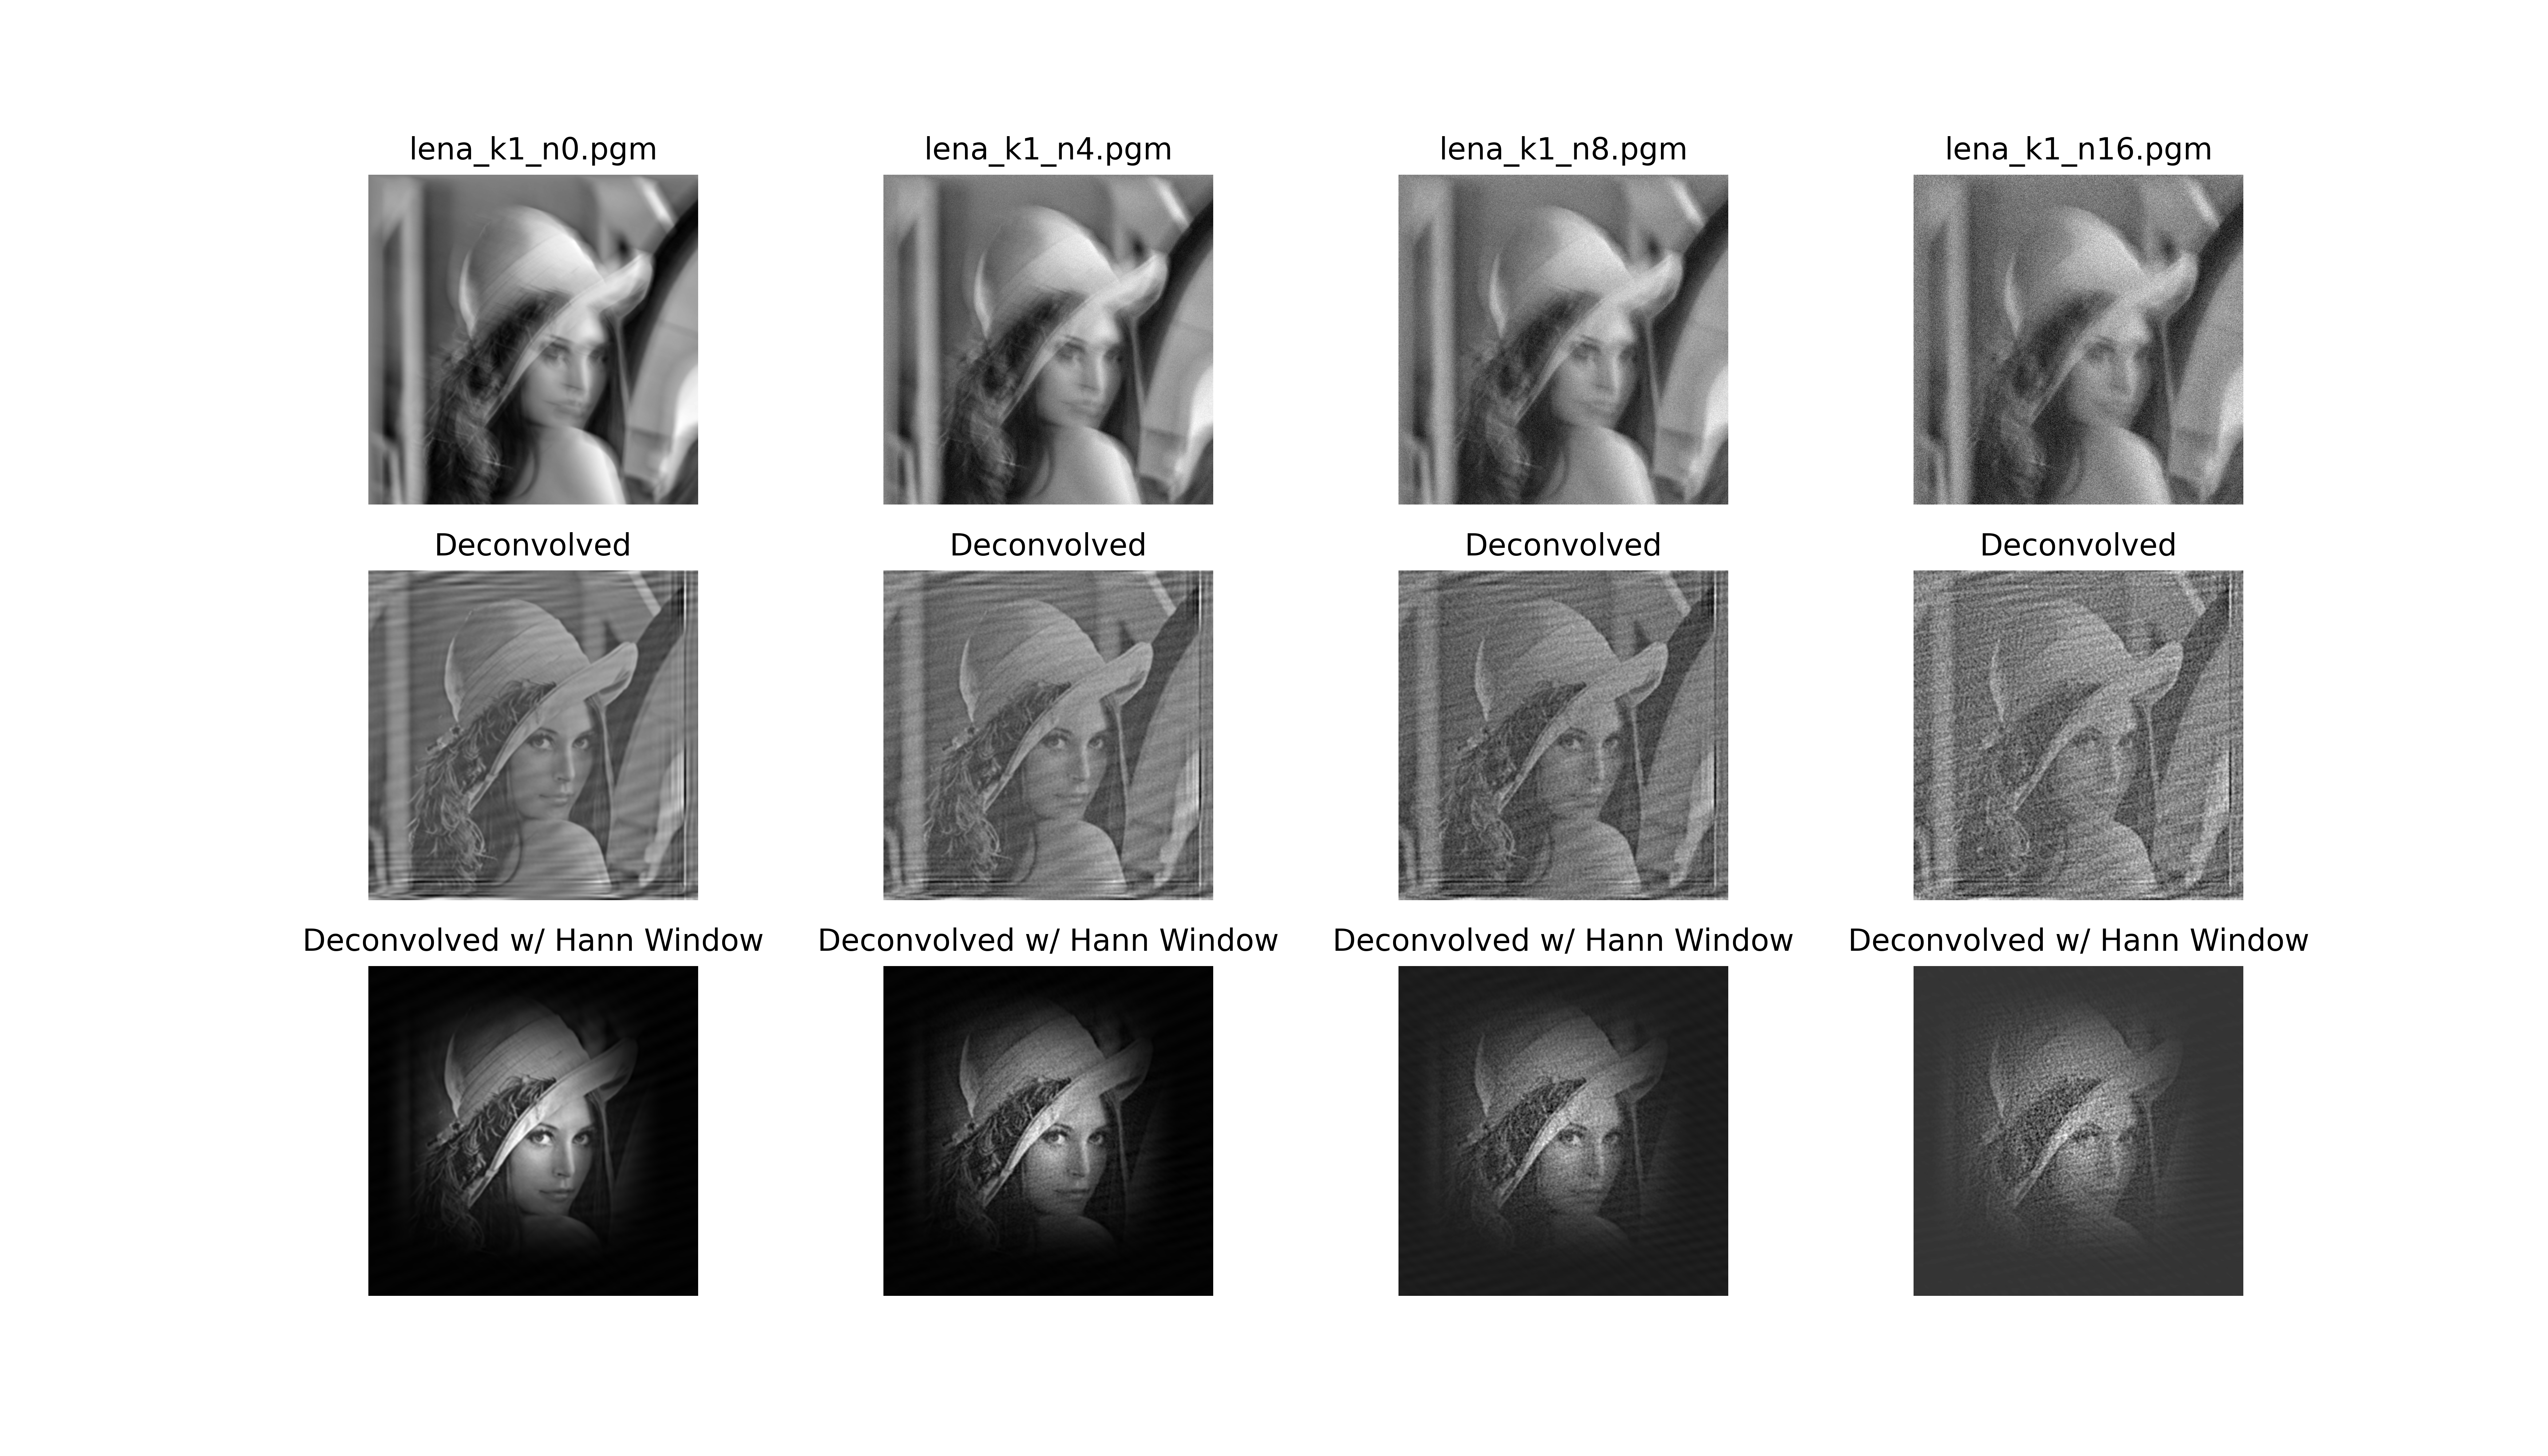
\includegraphics[width=0.98\textwidth]{../ImageDeconvolution/Images/lena_k1_deconvolved.png}
    \caption{Wiener deconvolution applied to the Lena images convolved with the first kernel.}
    \label{fig:lena-1}
\end{figure}

We can see that the deconvolution yields fantastic results. I was shocked to see how clear Lena's face could become after 
the deconvolution. We do spot a typical problem of the Fourier Transform however. We can see that the deconvolution has
introduced some \textit{ringing} artifacts around the edges of the image, which is again as a result of the image being 
non-periodic. This can be fixed with windowing which I attempted to do using a Hann window in the last row. I wanted to see 
how different windows for the purpose of image restoration. The results are shown in Figure \ref{fig:lena-1-windowing}.

\begin{figure}[H]
    \centering
    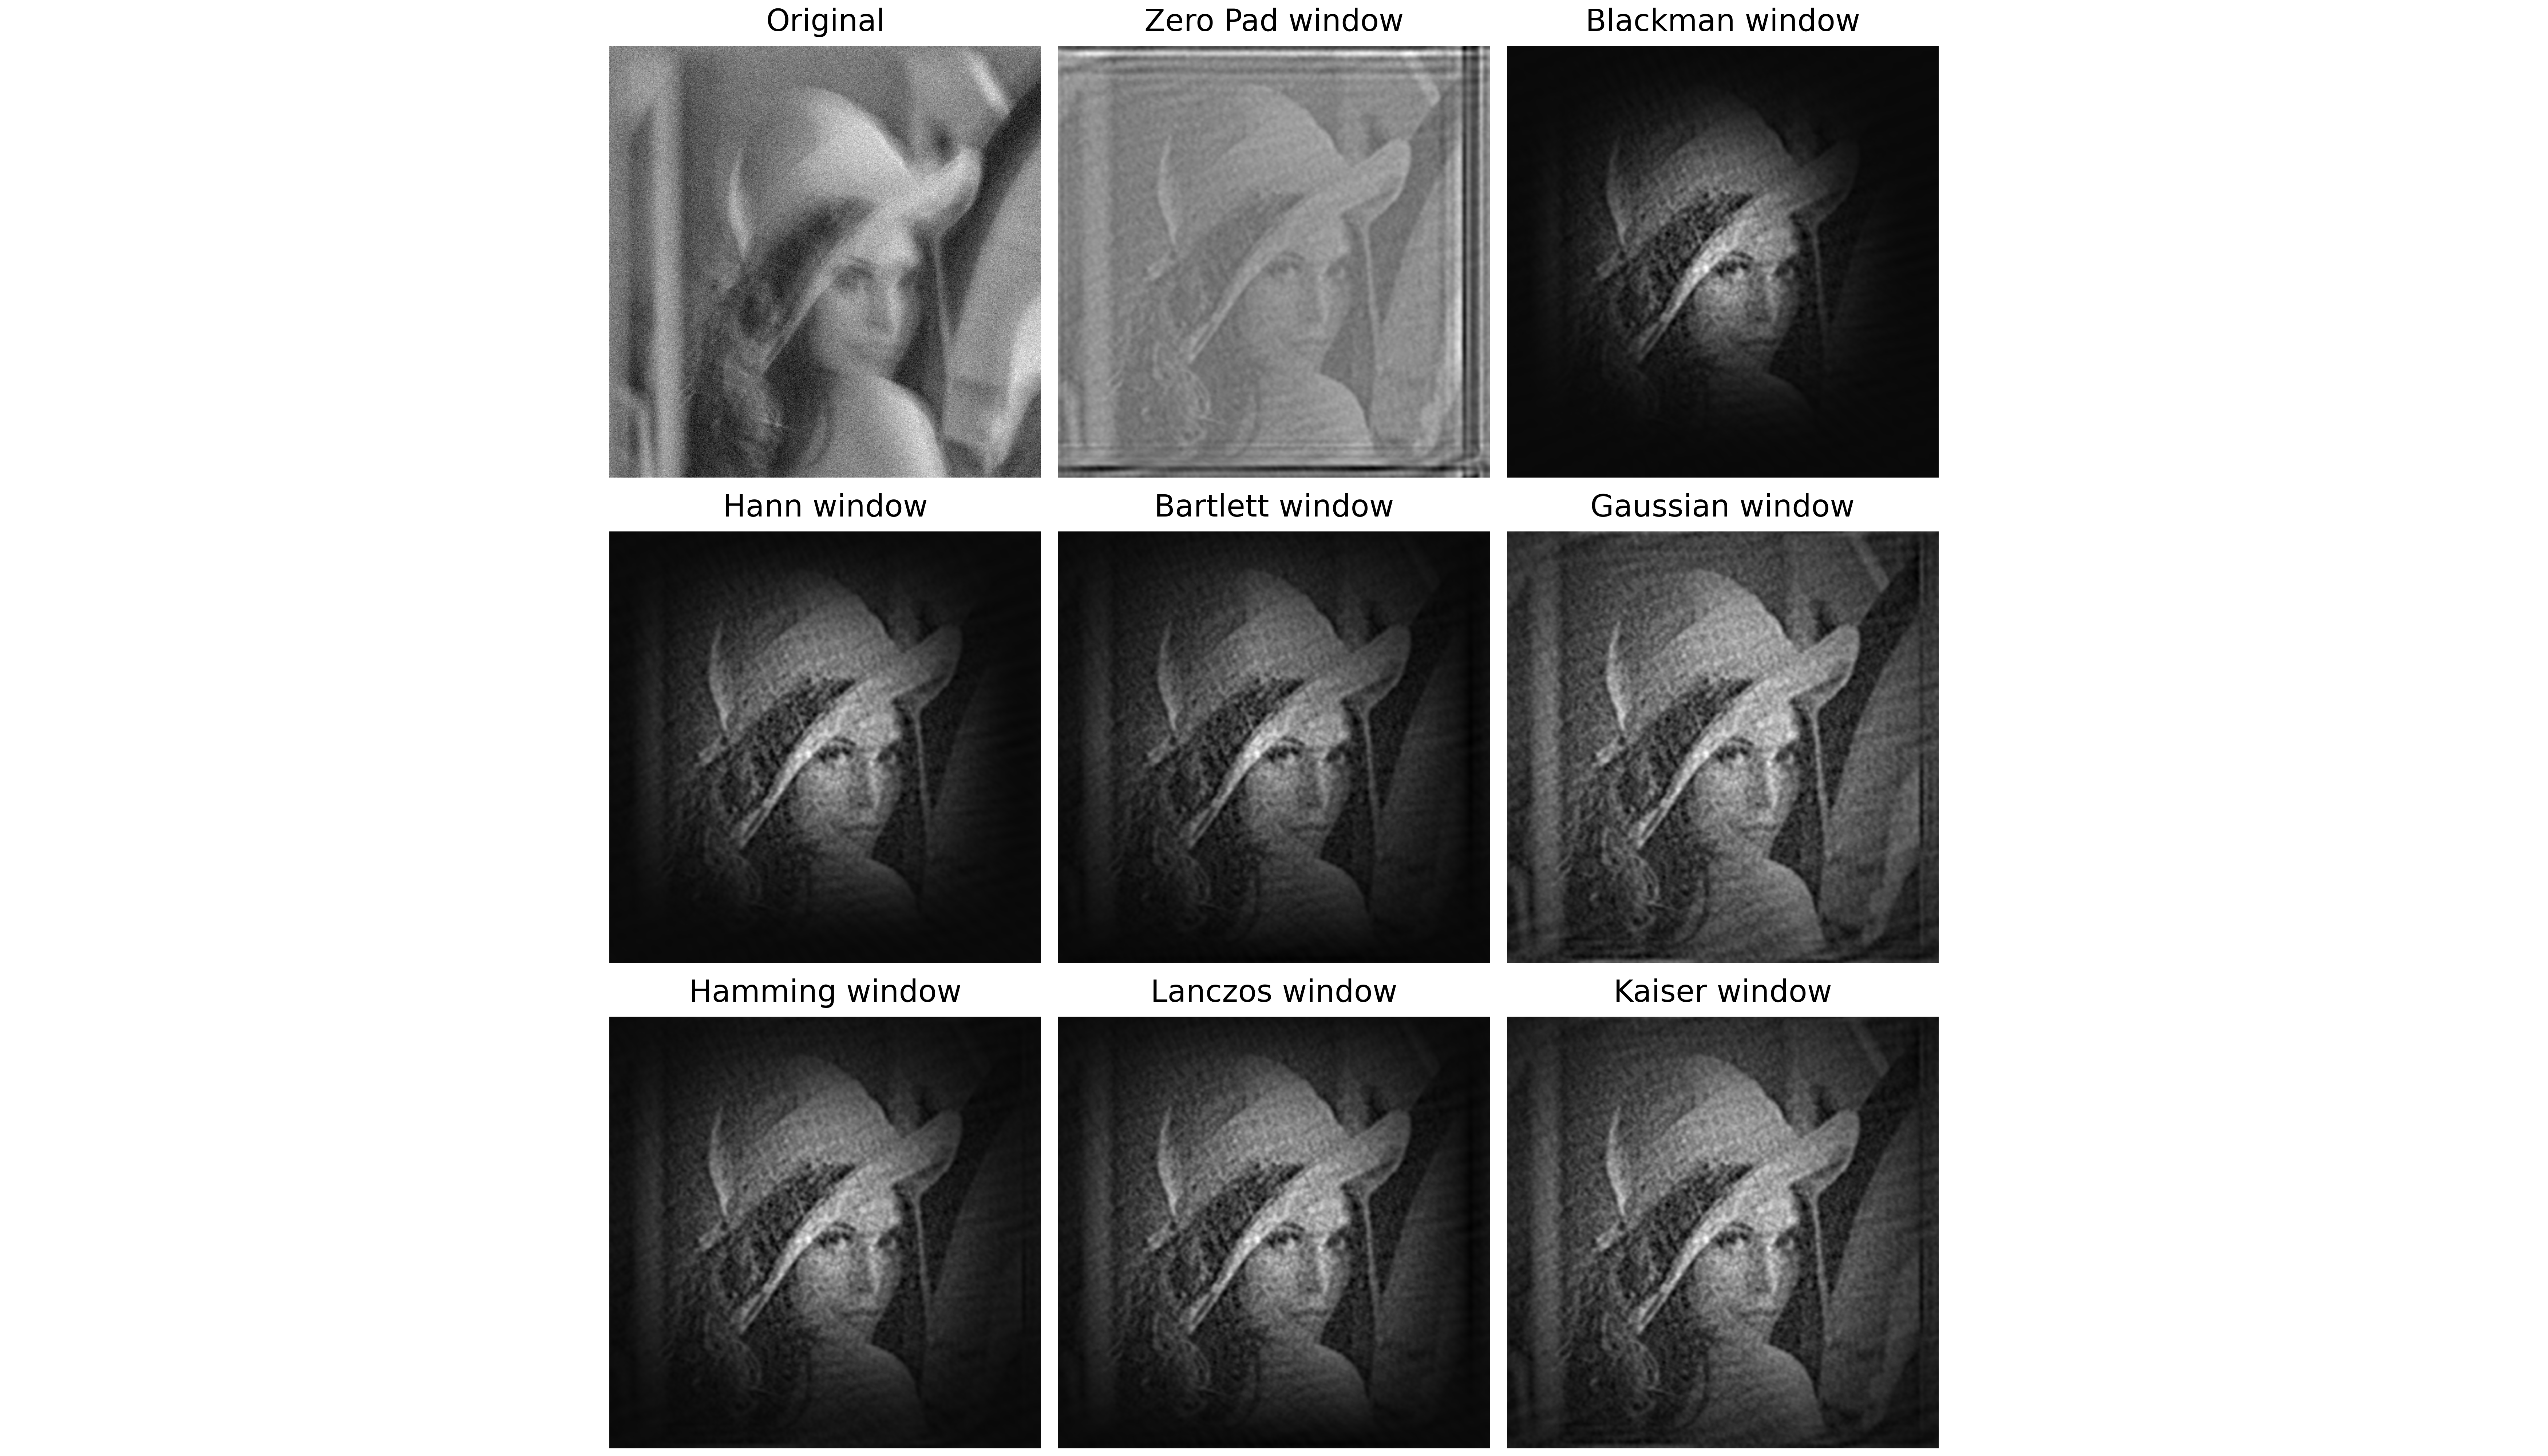
\includegraphics[width=0.98\textwidth]{../ImageDeconvolution/Images/lena_k1_n16_windows.png}
    \caption{Wiener deconvolution applied to the Lena images convolved with the first kernel with different windowing functions.}
    \label{fig:lena-1-windowing}
\end{figure}

From this image we can come to the conclusion that the best windows for the purpose of image restoration are the Gaussian 
and Kaiser windows. They both do a good job at removing the ringing artifacts without introducing vingetting too much. The other 
windows might remove the artifacts well but distort the image in their own way in the process. The added Gaussian noise 
really does a number on the image making it much harder to restore. \\

Moving on to the second kernel that represents \textit{motion blur} we can see the results in Figure \ref{fig:lena-2}.

\begin{figure}[H]
    \centering
    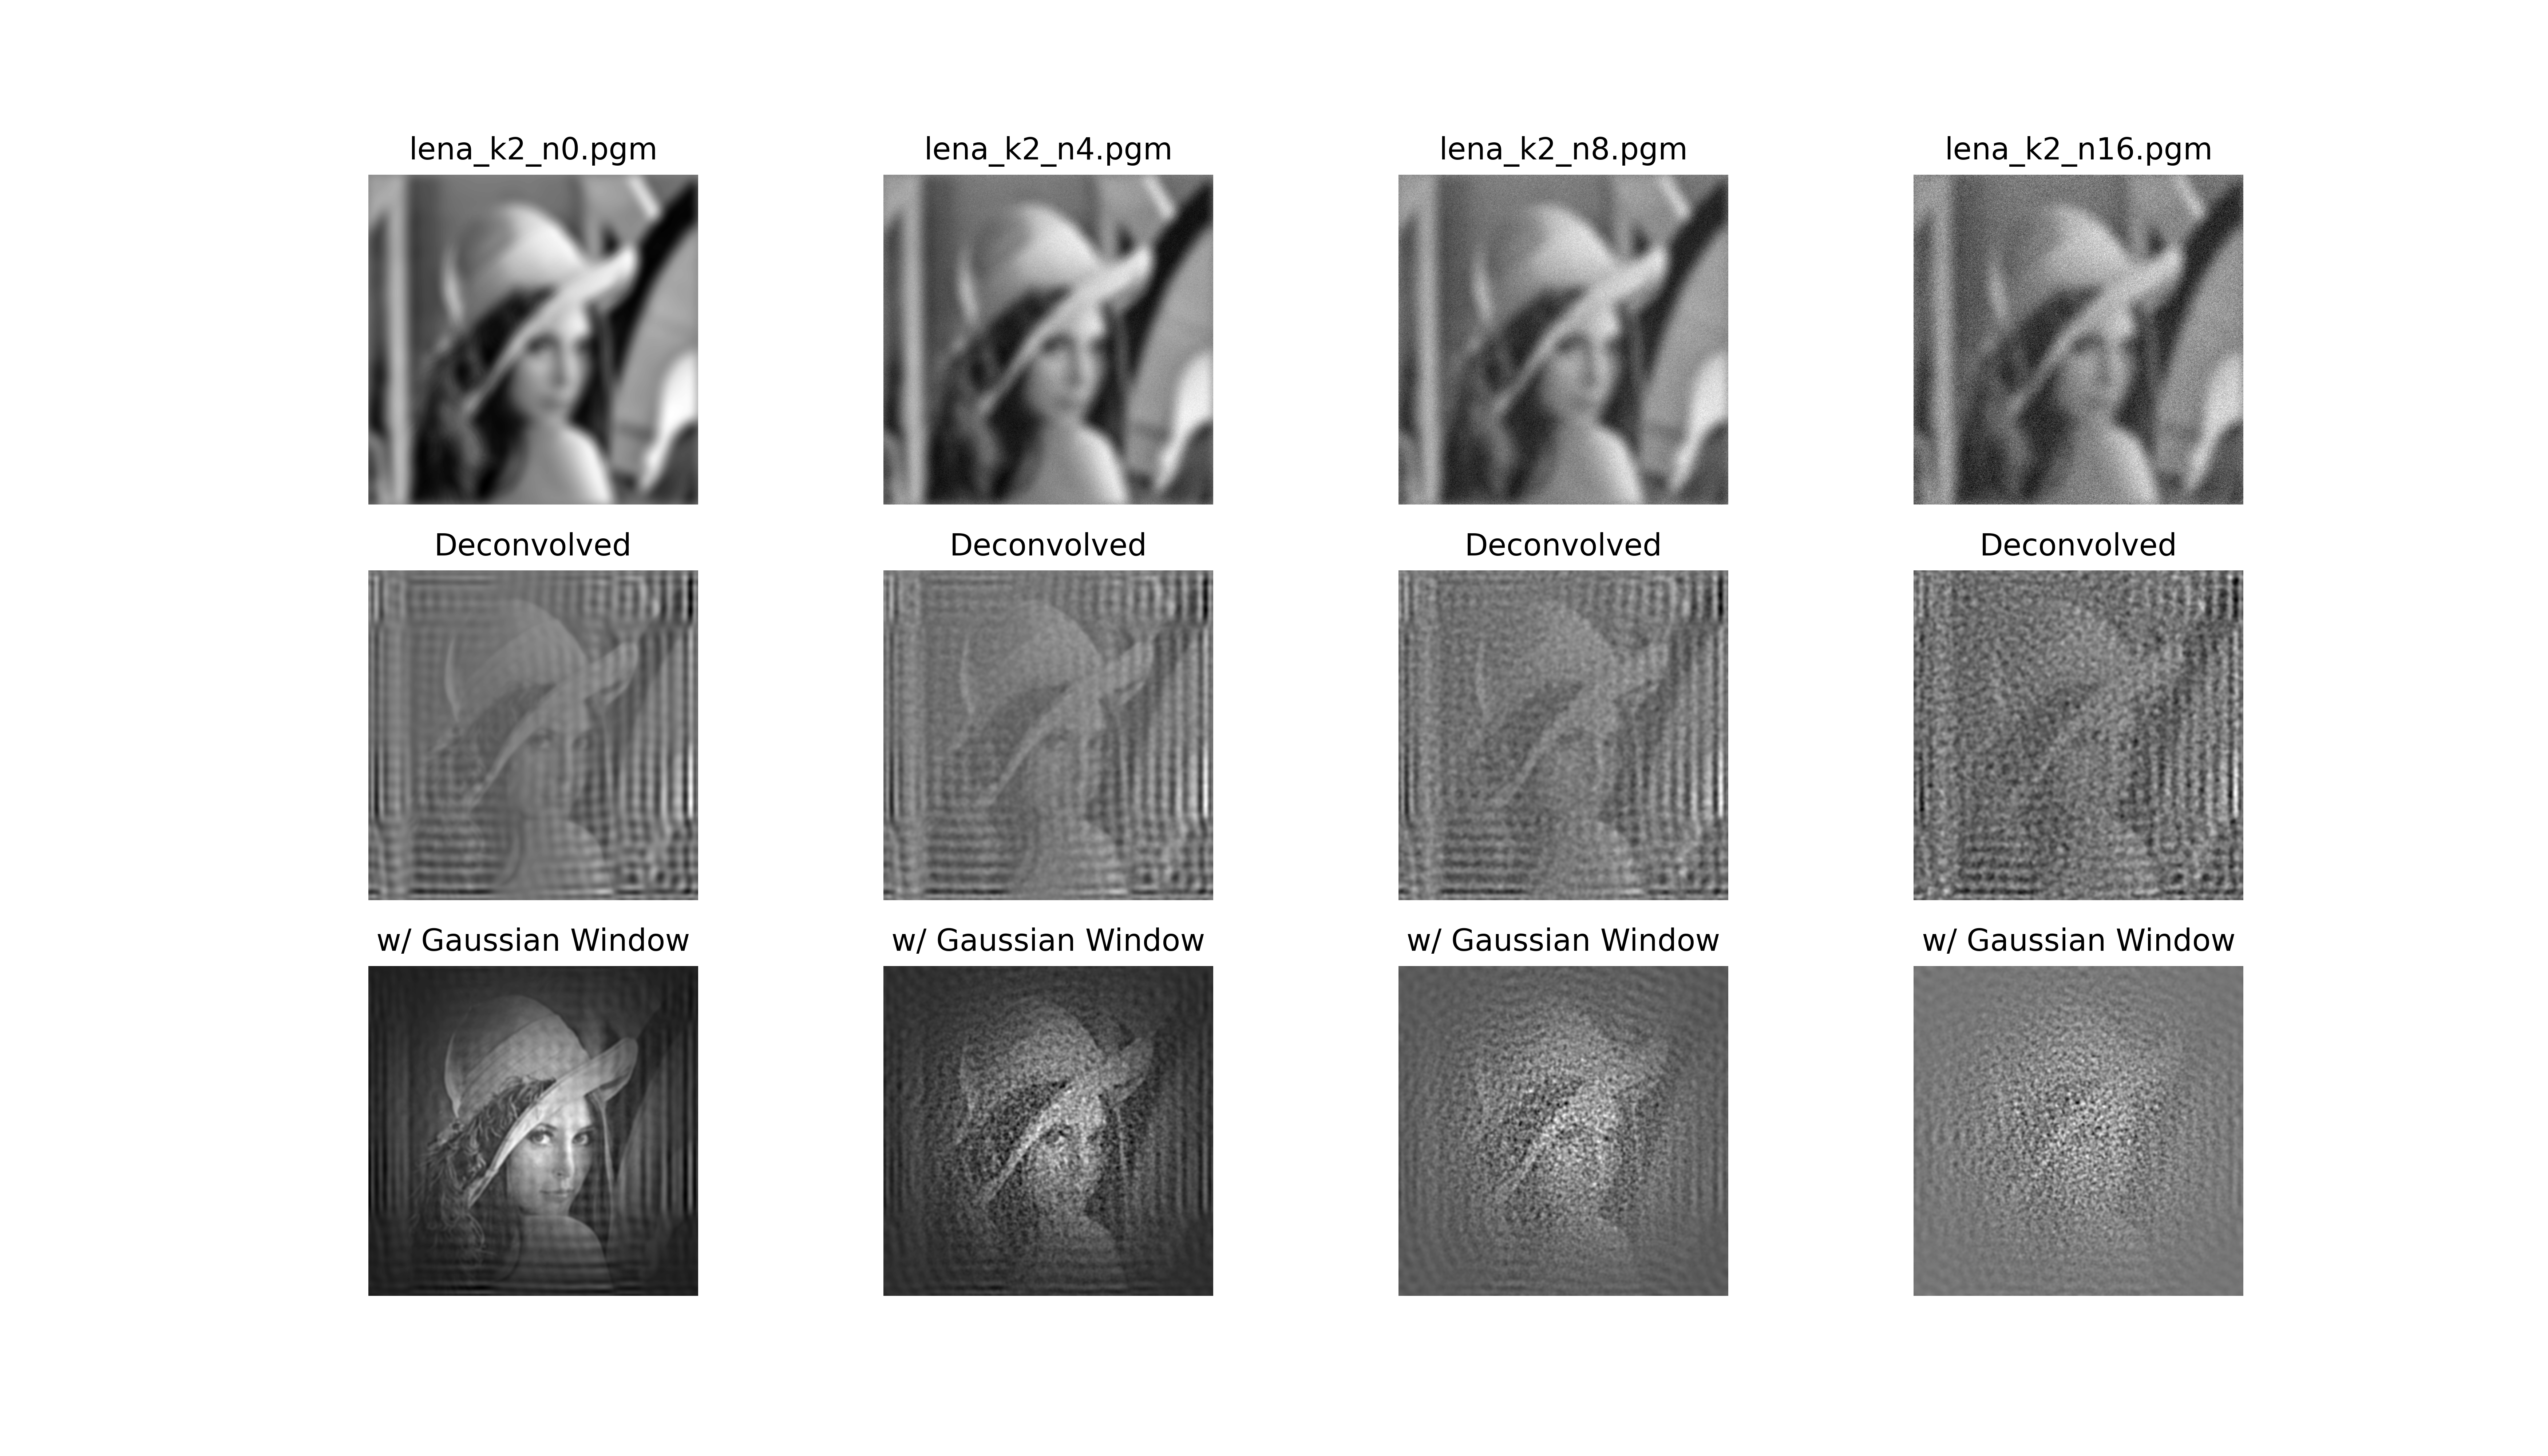
\includegraphics[width=0.98\textwidth]{../ImageDeconvolution/Images/lena_k2_deconvolved.png}
    \caption{Wiener deconvolution applied to the Lena images convolved with the second kernel.}
    \label{fig:lena-2}
\end{figure}

The results are decent but it's clear that this kernel is much harder to deconvolve. The motion blur is much more prominent
and the deconvolution can't really remove it. At higher values of added Gaussian noise the image becomes more or less 
unrecoverable. The deconvolution introduces some heavy periodic perturbations to the image as a result of leakage effects.
I investigated on how I could mitigate this using frequency domain filtering. In the end I settled for a phase unwrapping 
algorithm by Miguel Arevallilo Herráez et al. which is described in \ref{Herraez:02}. The results are shown in Figure
\ref{fig:lena-2-unwrapping}, where I've also included the results of the windowed deconvolution for comparison.

\begin{figure}[H]
    \centering
    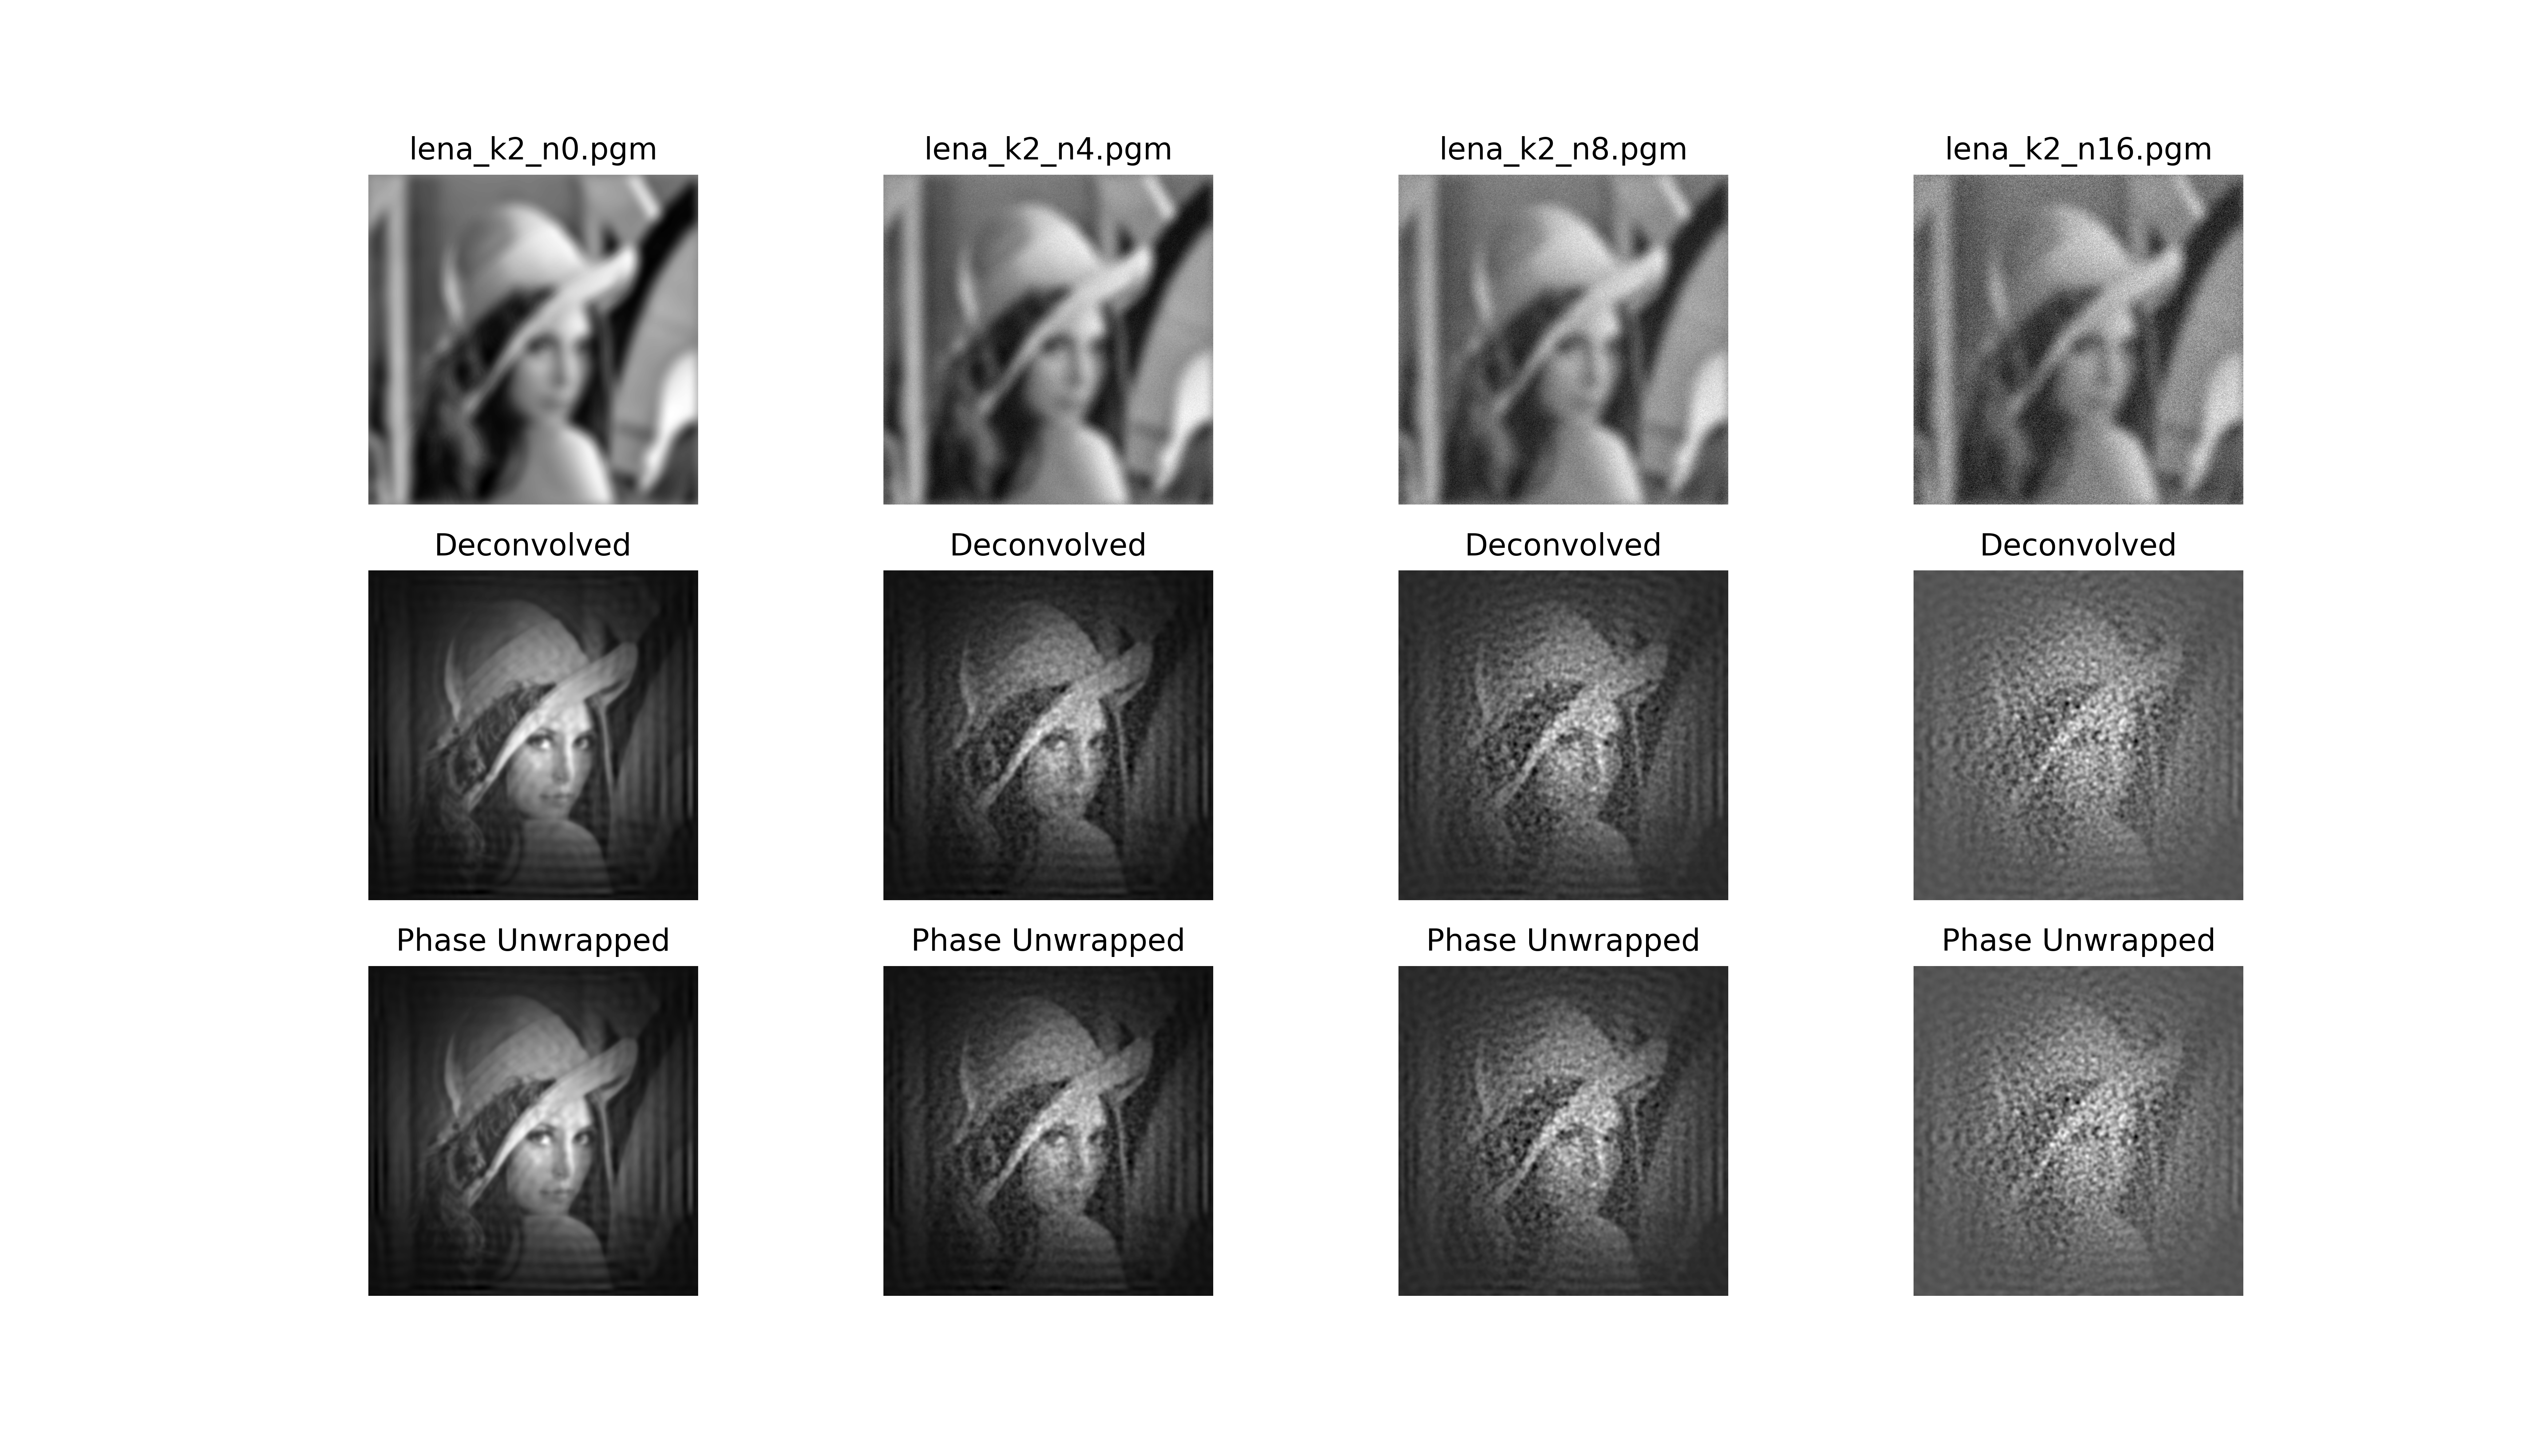
\includegraphics[width=0.98\textwidth]{../ImageDeconvolution/Images/lena_k2_deconvolved_noperiodic.png}
    \caption{Wiener deconvolution applied to the Lena images convolved with the second kernel with phase unwrapping.}
    \label{fig:lena-2-unwrapping}
\end{figure}

I also experimented myself with just mindlessly editing the values of the Fourier Transform of the image. I tried to
remove the periodic perturbations by setting the values of the Fourier Transform to the average of the values in the
spectrum. The results are shown in Figure \ref{fig:lena-2-averaging}.

\begin{figure}[H]
    \centering
    \includegraphics[width=0.98\textwidth]{../ImageDeconvolution/Images/lena_k2_deconvolved_spectra.png}
    \caption{Lena images convolved with the second kernel with hand-edited Fourier Transform.}
    \label{fig:lena-2-averaging}
\end{figure}

The results seem horrible. I can't seem to identify which part of the spectrum contains the periodic perturbations.
I made the image darker, blurrier and I managed to make Lena look a bit more masculine. Moving on to the last 
kernel that represents \textit{a diffraction grating} we can see the results in Figure \ref{fig:lena-3}.

\begin{figure}[H]
    \centering
    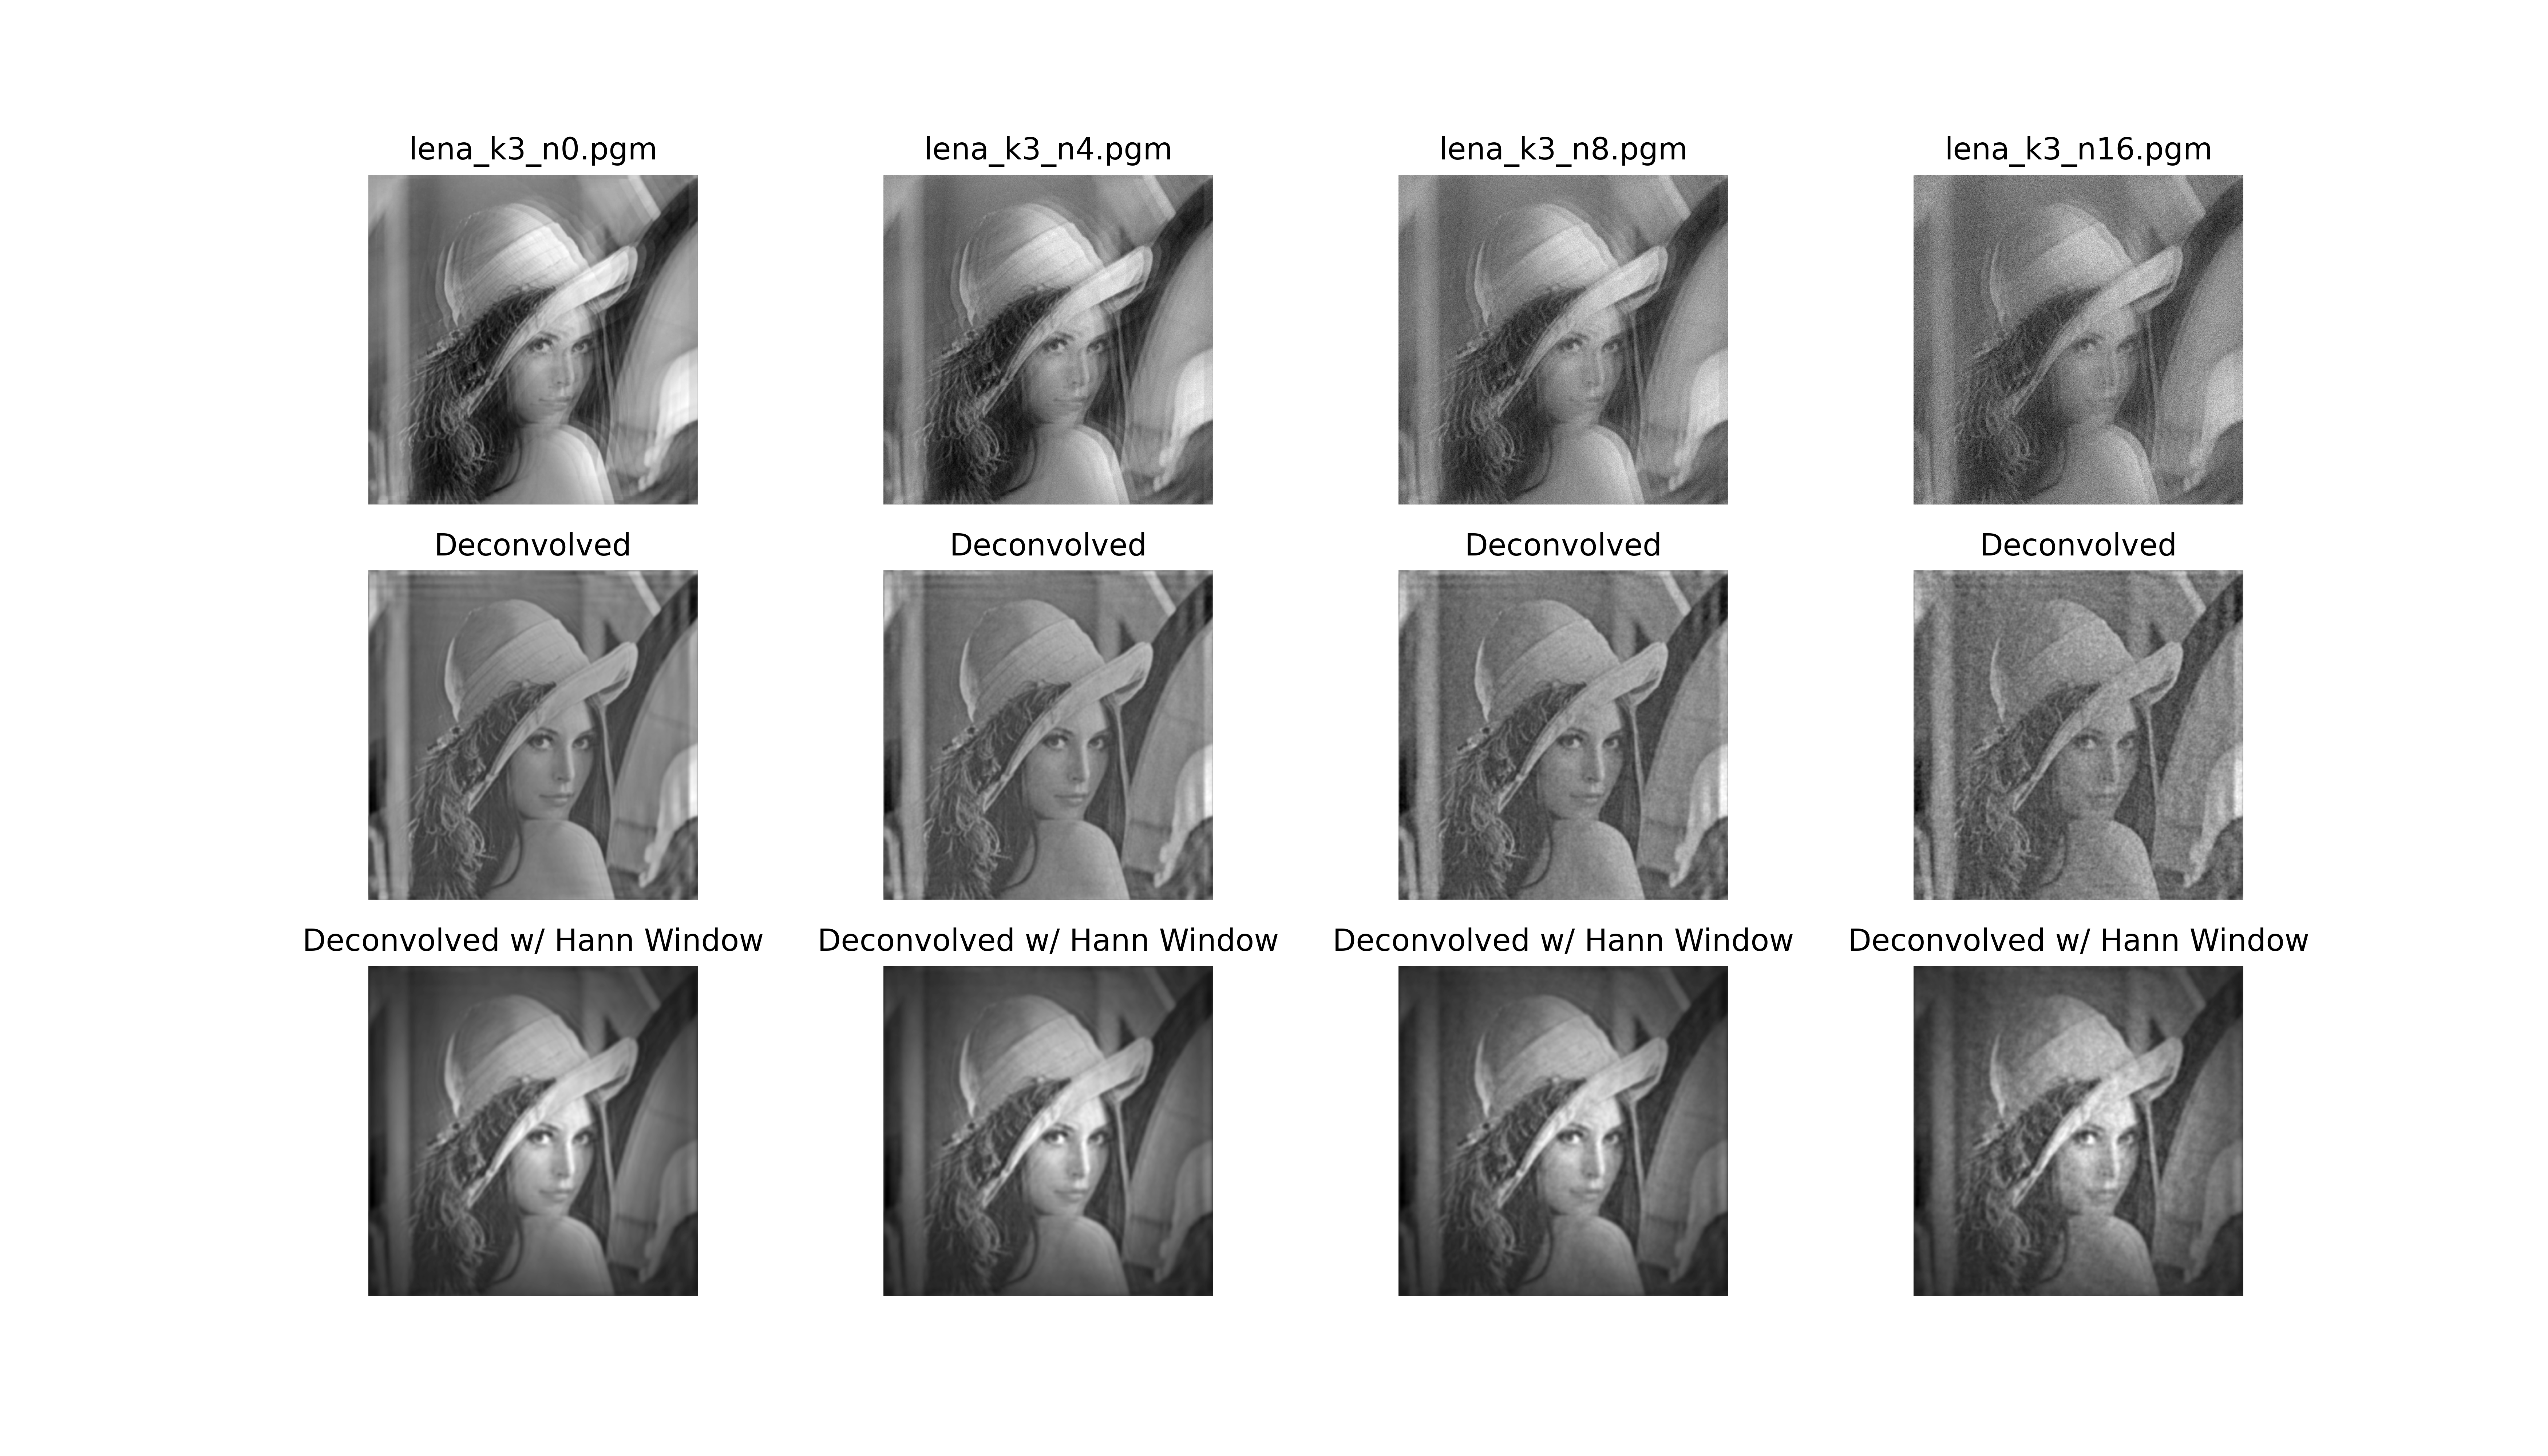
\includegraphics[width=0.98\textwidth]{../ImageDeconvolution/Images/lena_k3_deconvolved.png}
    \caption{Wiener deconvolution applied to the Lena images convolved with the third kernel.}
    \label{fig:lena-3}
\end{figure}

\section{Conclusion and Comments}

% Add references
% \newpage
% \bibliographystyle{unsrt}
% \bibliography{mod110}

% End document

\newpage
\section{Large Figures}

\begin{figure}[H]
    \centering
    \includegraphics[width=0.98\textwidth]{../WienerFilter/Images/reconstructed-signal1.dat.png}
    \caption{Wiener filter applied to the signal \texttt{signal1.dat}.}
    \label{fig:wiener-filter-1}
\end{figure}

\begin{figure}[H]
    \centering
    \includegraphics[width=0.98\textwidth]{../WienerFilter/Images/reconstructed-signal2.dat.png}
    \caption{Wiener filter applied to the signal \texttt{signal2.dat}.}
    \label{fig:wiener-filter-2}
\end{figure}

\begin{figure}[H]
    \centering
    \includegraphics[width=0.98\textwidth]{../WienerFilter/Images/reconstructed-signal3.dat.png}
    \caption{Wiener filter applied to the signal \texttt{signal3.dat}.}
    \label{fig:wiener-filter-3}
\end{figure}


\begin{figure}[H]
    \centering
    \includegraphics[width=0.98\textwidth]{../WienerFilter/Images/multiple-signal1.dat.png}
    \caption{Wiener filter applied consecutively to the signal \texttt{signal1.dat}.}
    \label{fig:wiener-filter-1-2}
\end{figure}

\begin{figure}[H]
    \centering
    \includegraphics[width=0.98\textwidth]{../WienerFilter/Images/multiple-signal2.dat.png}
    \caption{Wiener filter applied consecutively to the signal \texttt{signal2.dat}.}
    \label{fig:wiener-filter-2-2}
\end{figure}

\begin{figure}[H]
    \centering
    \includegraphics[width=0.98\textwidth]{../WienerFilter/Images/multiple-signal3.dat.png}
    \caption{Wiener filter applied consecutively to the signal \texttt{signal3.dat}.}
    \label{fig:wiener-filter-3-2}
\end{figure}


\begin{figure}[H]
    \centering
    \includegraphics[width=0.98\textwidth]{../WienerFilter/Images/filters-signal1.dat.png}
    \caption{Wiener filter and other filters applied to the signal \texttt{signal1.dat}.}
    \label{fig:other-filters-1}
\end{figure}

\begin{figure}[H]
    \centering
    \includegraphics[width=0.98\textwidth]{../WienerFilter/Images/filters-signal2.dat.png}
    \caption{Wiener filter and other filters applied to the signal \texttt{signal2.dat}.}
    \label{fig:other-filters-2}
\end{figure}

\begin{figure}[H]
    \centering
    \includegraphics[width=0.98\textwidth]{../WienerFilter/Images/filters-signal3.dat.png}
    \caption{Wiener filter and other filters applied to the signal \texttt{signal3.dat}.}
    \label{fig:other-filters-3}
\end{figure}

\end{document}
